\documentclass[aspectratio=169,10pt]{beamer}

% Theme & Styling
\usetheme{Madrid}
\usecolortheme{whale}

% -----------------------------------------------------------------------------
% Elegant Obsidian / Dark Aesthetic Palette (Grant Sanderson 3Blue1Brown Style)
% -----------------------------------------------------------------------------
\definecolor{DarkCanvas}{RGB}{12, 16, 24}      % Deep obsidian canvas
\definecolor{DarkBox}{RGB}{20, 27, 40}         % Translucent dark card
\definecolor{DarkBoxInner}{RGB}{26, 36, 54}    % Accent box background
\definecolor{LuminousGold}{RGB}{245, 190, 60}  % Vibrant Gold / ITB Gold
\definecolor{ElectricBlue}{RGB}{80, 165, 250}  % Luminous Sky Blue
\definecolor{TealCyan}{RGB}{45, 212, 191}      % Cyan / Teal
\definecolor{EmeraldGreen}{RGB}{52, 211, 153}  % High-contrast green (Maks/Min)
\definecolor{CoralRose}{RGB}{251, 113, 133}    % High-contrast rose (Peringatan/Ekstrem)
\definecolor{SoftGray}{RGB}{200, 210, 225}     % Readable muted text

% Apply Dark Colors to Beamer Elements
\setbeamercolor{background canvas}{bg=DarkCanvas}
\setbeamercolor{normal text}{fg=white}
\setbeamercolor{structure}{fg=ElectricBlue}
\setbeamercolor{title}{fg=white,bg=DarkBox}
\setbeamercolor{frametitle}{fg=LuminousGold,bg=DarkBox}
\setbeamercolor{footline}{fg=SoftGray!70,bg=DarkCanvas}
\setbeamercolor{headline}{fg=SoftGray!70,bg=DarkCanvas}

% Block Styles in Dark Theme
\setbeamercolor{block title}{fg=white,bg=ElectricBlue!45!black}
\setbeamercolor{block body}{fg=white,bg=DarkBox}
\setbeamercolor{block title example}{fg=white,bg=EmeraldGreen!40!black}
\setbeamercolor{block body example}{fg=white,bg=DarkBox}
\setbeamercolor{block title alerted}{fg=white,bg=CoralRose!45!black}
\setbeamercolor{block body alerted}{fg=white,bg=DarkBox}

% Lists & Numbering
\setbeamercolor{item}{fg=LuminousGold}
\setbeamercolor{subitem}{fg=TealCyan}
\setbeamercolor{enumerate item}{fg=LuminousGold}
\setbeamercolor{enumerate subitem}{fg=TealCyan}

% Packages
\usepackage[utf8]{inputenc}
\usepackage{amsmath,amssymb}
\usepackage{graphicx}
\usepackage{hyperref}
\usepackage{multimedia}
\usepackage{tikz}

\hypersetup{
    colorlinks=true,
    linkcolor=TealCyan,
    urlcolor=ElectricBlue
}

\title[MA1101 Matematika I]{MA1101 Matematika I --- Bab 3: Penggunaan Turunan}
\subtitle{Subtopik 3.1: Maksimum dan Minimum (\textit{Maximum and Minimum Values})}
\author[FMIPA ITB]{Tim Pengajar MA1101}
\institute[ITB]{Fakultas Matematika dan Ilmu Pengetahuan Alam\\Institut Teknologi Bandung}
\date{Semester 1 Tahun Akademik 2026/2027}

\begin{document}

% -------------------------------------------------------------
% Slide 1: Judul
% -------------------------------------------------------------
\begin{frame}
    \titlepage
\end{frame}

% -------------------------------------------------------------
% Slide 2: Motivasi & Tantangan Sokratik (The Pique)
% -------------------------------------------------------------
\begin{frame}{Tantangan Awal: Mencari Puncak dan Lembah Tertinggi}
    \begin{columns}[T]
        \begin{column}{0.55\textwidth}
            \begin{block}{Motivasi Optimasi}
                \begin{itemize}
                    \item Mencari kondisi terbaik: keuntungan puncak, efisiensi energi, atau kapasitas optimal.
                    \item Secara matematis: menentukan \textbf{maksimum mutlak} dan \textbf{minimum mutlak} dari fungsi $y = f(x)$.
                \end{itemize}
            \end{block}

            \vspace{0.1cm}
            \begin{alertblock}{Pertanyaan Sokratik}
                Jika mendaki kurva $y = f(x)$ pada domain tertutup $[a, b]$, di manakah puncak dan lembah dapat berada?\\
                Apakah selalu saat garis singgung mendatar ($f'=0$)? Bagaimana dengan batas selang dan titik sudut tajam?
            \end{alertblock}
        \end{column}

        \begin{column}{0.42\textwidth}
            \centering
            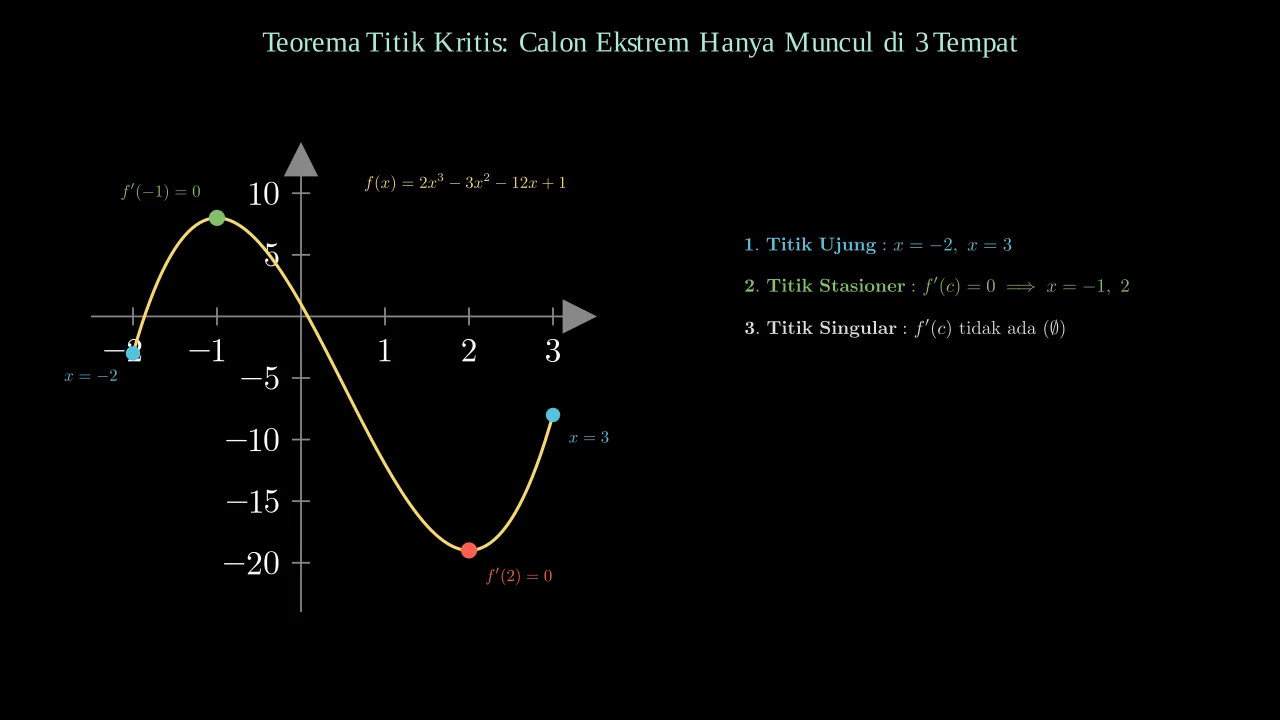
\includegraphics[width=\textwidth]{keyframe_maksimin.png}\\
            \vspace{0.1cm}
            {\scriptsize \color{SoftGray} \textit{Eksplorasi Kurva: Kandidat puncak \& lembah pada domain $[a, b]$}}
        \end{column}
    \end{columns}
\end{frame}

% -------------------------------------------------------------
% Slide 3: Teorema Nilai Ekstrem (Extreme Value Theorem / EVT)
% -------------------------------------------------------------
\begin{frame}{Teorema Nilai Ekstrem (\textit{Extreme Value Theorem} / EVT)}
    \begin{columns}[T]
        \begin{column}{0.48\textwidth}
            \begin{block}{Definisi Nilai Ekstrem Mutlak}
                Misalkan $S$ adalah daerah asal (\textit{domain}) fungsi $f$:
                \begin{itemize}
                    \item $f(c)$ adalah \textbf{Maksimum Mutlak} jika:
                    \[
                        f(c) \ge f(x) \quad \text{untuk semua } x \in S
                    \]
                    \item $f(c)$ adalah \textbf{Minimum Mutlak} jika:
                    \[
                        f(c) \le f(x) \quad \text{untuk semua } x \in S
                    \]
                \end{itemize}
            \end{block}
        \end{column}

        \begin{column}{0.48\textwidth}
            \begin{exampleblock}{Teorema Nilai Ekstrem (EVT)}
                Jika fungsi $f$ \textbf{kontinu} pada selang tertutup $[a, b]$, maka $f$ \textbf{pasti} mencapai nilai maksimum mutlak dan nilai minimum mutlak pada $[a, b]$.
            \end{exampleblock}

            \begin{alertblock}{Dua Syarat Mutlak EVT}
                \begin{enumerate}
                    \item Fungsi $f$ harus \textbf{kontinu} pada $[a, b]$.
                    \item Selang domain harus \textbf{tertutup} $[a, b]$.
                \end{enumerate}
                {\scriptsize \color{SoftGray} \textit{Jika salah satu syarat gagal, nilai ekstrem mutlak tidak dijamin ada!}}
            \end{alertblock}
        \end{column}
    \end{columns}
\end{frame}

% -------------------------------------------------------------
% Slide 4: Tiga "Habitat" Titik Kritis
% -------------------------------------------------------------
\begin{frame}{Teorema Titik Kritis (Fermat): Tiga "Habitat" Calon Ekstrem}
    \begin{block}{Teorema Titik Kritis}
        Misalkan $f$ terdefinisi pada selang $I$ yang memuat titik $c$. Jika $f(c)$ adalah nilai ekstrem, maka $c$ \textbf{harus berupa titik kritis}, yaitu salah satu dari tiga jenis berikut:
    \end{block}

    \vspace{0.15cm}
    \begin{columns}[T]
        \begin{column}{0.32\textwidth}
            \begin{block}{1. Titik Ujung}
                Ujung-ujung selang domain:
                \[
                    x = a \quad \text{atau} \quad x = b
                \]
                {\scriptsize \color{SoftGray} \textit{Tempat penjelajahan domain berhenti secara alami.}}
            \end{block}
        \end{column}

        \begin{column}{0.32\textwidth}
            \begin{exampleblock}{2. Titik Stasioner}
                Titik di mana turunan bernilai nol:
                \[
                    \mathbf{f'(c) = 0}
                \]
                {\scriptsize \color{SoftGray} \textit{Garis singgung mendatar horizontal (puncak bukit / dasar lembah mulus).}}
            \end{exampleblock}
        \end{column}

        \begin{column}{0.32\textwidth}
            \begin{alertblock}{3. Titik Singular}
                Titik di mana turunan \textbf{tidak ada}:
                \[
                    \mathbf{f'(c)\ \text{tidak ada}}
                \]
                {\scriptsize \color{SoftGray} \textit{Titik sudut tajam/pojok (misal $|x|$) atau garis singgung vertikal ($x^{2/3}$).}}
            \end{alertblock}
        \end{column}
    \end{columns}
\end{frame}

% -------------------------------------------------------------
% Slide 5: Simulasi Video Interaktif
% -------------------------------------------------------------
\begin{frame}{Simulasi Dinamis: Pelacakan Titik Kritis \& EVT}
    \centering
    % Embedded video untuk presenter (Pympress / PDFPC / Okular)
    \movie[width=9.6cm,height=5.4cm,poster,showcontrols=true]{%
        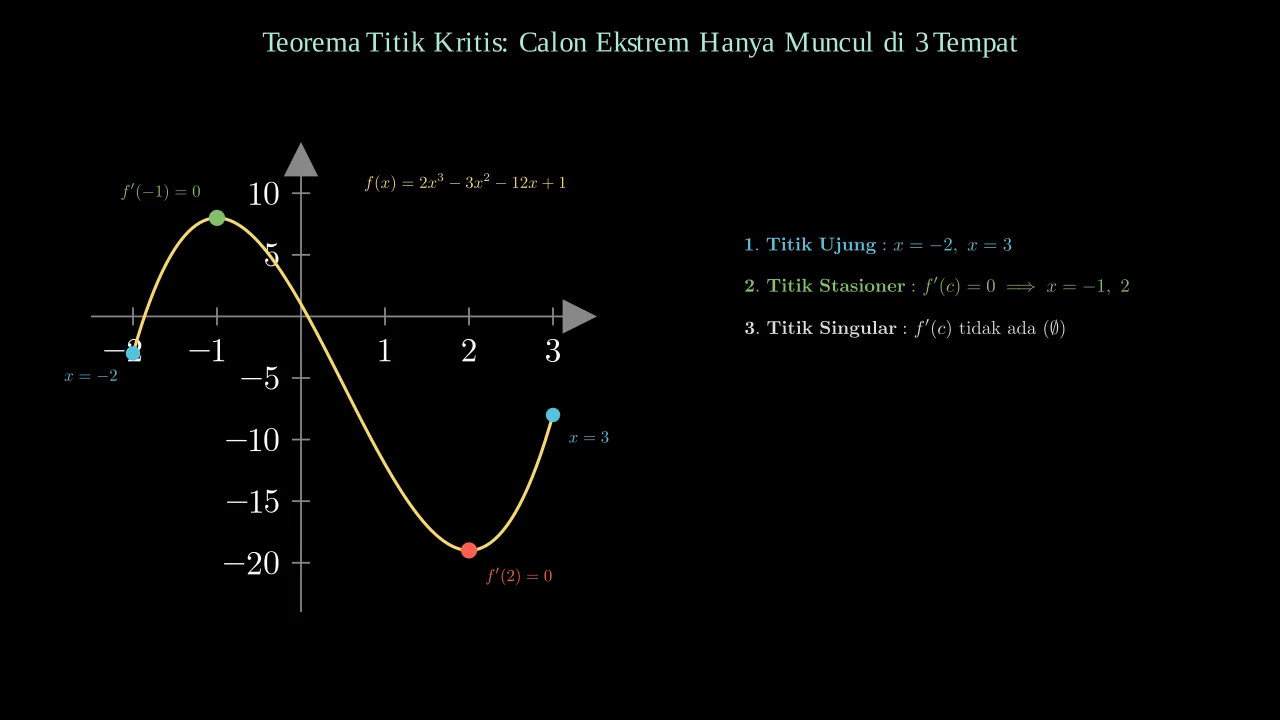
\includegraphics[height=0.55\textheight]{keyframe_maksimin.png}%
    }{MaximumMinimumScene.ogv}
    
    \vspace{0.2cm}
    \href{file:MaximumMinimumScene.mp4}{%
        \beamergotobutton{\normalsize $\blacktriangleright$ Putar Video (\texttt{MaximumMinimumScene.mp4})}%
    }
    
    \vspace{0.15cm}
    {\scriptsize \color{SoftGray} \textit{Klik poster untuk memutar langsung di Pympress/Okular, atau klik tombol untuk membuka di MPV/VLC.}}
\end{frame}

% -------------------------------------------------------------
% Slide 6: Metode Selang Tertutup (Closed Interval Method)
% -------------------------------------------------------------
\begin{frame}{Metode Selang Tertutup (\textit{Closed Interval Method})}
    Untuk menentukan nilai maksimum mutlak dan minimum mutlak fungsi kontinu $f$ pada $[a, b]$:

    \vspace{0.15cm}
    \begin{columns}[T]
        \begin{column}{0.48\textwidth}
            \begin{block}{Langkah 1: Cari Titik Kritis di Dalam $(a, b)$}
                \begin{itemize}
                    \item Selesaikan persamaan $f'(x) = 0$ (titik stasioner).
                    \item Cari nilai $x$ di mana $f'(x)$ tidak terdefinisi (titik singular).
                    \item \textbf{Perhatian:} Hanya ambil titik kritis yang berada di dalam selang buka $(a, b)$.
                \end{itemize}
            \end{block}

            \begin{block}{Langkah 2: Hitung Nilai Titik Kritis}
                Hitung nilai fungsi $f(c)$ untuk setiap titik kritis $c \in (a, b)$ yang ditemukan.
            \end{block}
        \end{column}

        \begin{column}{0.48\textwidth}
            \begin{block}{Langkah 3: Hitung Nilai Titik Ujung}
                Hitung nilai fungsi pada kedua ujung selang:
                \[
                    f(a) \quad \text{dan} \quad f(b)
                \]
            \end{block}

            \begin{alertblock}{Langkah 4: Bandingkan Seluruh Nilai}
                Bandingkan semua nilai dari Langkah 2 dan 3:
                \begin{itemize}
                    \item Nilai \textbf{terbesar} adalah \textbf{Maksimum Mutlak}.
                    \item Nilai \textbf{terkecil} adalah \textbf{Minimum Mutlak}.
                \end{itemize}
            \end{alertblock}
        \end{column}
    \end{columns}
\end{frame}

% -------------------------------------------------------------
% Slide 7: Contoh Soal 1: Fungsi Polinomial Kubik
% -------------------------------------------------------------
\begin{frame}{Contoh Soal 1: Fungsi Polinomial Kubik}
    \textbf{Soal}: Tentukan nilai maksimum mutlak dan minimum mutlak dari:
    \[
        f(x) = 2x^3 - 3x^2 - 12x + 1 \quad \text{pada selang tertutup } [-2, 3]
    \]

    \pause
    \begin{columns}[T]
        \begin{column}{0.48\textwidth}
            \begin{block}{Langkah 1: Turunan \& Titik Kritis}
                Fungsi $f$ kontinu pada $[-2, 3]$.
                \[
                    f'(x) = 6x^2 - 6x - 12
                \]
                Faktorkan untuk mencari pembuat nol:
                \[
                    6(x^2 - x - 2) = 6(x - 2)(x + 1) = 0
                \]
                Diperoleh dua titik stasioner:
                \[
                    x = -1 \quad \text{dan} \quad x = 2
                \]
                {\scriptsize \color{SoftGray} (Keduanya berada di dalam selang buka $(-2, 3)$).}
            \end{block}
        \end{column}

        \begin{column}{0.48\textwidth}
            \begin{exampleblock}{Langkah 2 \& 3: Evaluasi Nilai Fungsi}
                Hitung nilai fungsi pada setiap kandidat titik kritis:
                \begin{itemize}
                    \item Ujung $x = -2 \implies f(-2) = \mathbf{-3}$
                    \item Stasioner $x = -1 \implies f(-1) = \mathbf{8}$
                    \item Stasioner $x = 2 \implies f(2) = \mathbf{-19}$
                    \item Ujung $x = 3 \implies f(3) = \mathbf{-8}$
                \end{itemize}
            \end{exampleblock}

            \begin{alertblock}{Kesimpulan Akhir}
                $\text{Maksimum Mutlak} = \mathbf{8}$ (tercapai di $x = -1$).\\
                $\text{Minimum Mutlak} = \mathbf{-19}$ (tercapai di $x = 2$).
            \end{alertblock}
        \end{column}
    \end{columns}
\end{frame}

% -------------------------------------------------------------
% Slide 8: Contoh Soal 2: Fungsi dengan Titik Singular
% -------------------------------------------------------------
\begin{frame}{Contoh Soal 2: Fungsi dengan Titik Singular}
    \textbf{Soal}: Tentukan nilai ekstrem mutlak dari $f(x) = x^{2/3}$ pada selang tertutup $[-1, 8]$.

    \pause
    \begin{columns}[T]
        \begin{column}{0.48\textwidth}
            \begin{block}{Langkah 1: Analisis Turunan}
                Turunkan fungsi $f(x) = x^{2/3}$:
                \[
                    f'(x) = \frac{2}{3} x^{-1/3} = \frac{2}{3\sqrt[3]{x}}
                \]
                \begin{itemize}
                    \item Pembilang $2 \neq 0 \implies f'(x) \neq 0$ (tidak ada titik stasioner).
                    \item Penyebut bernilai nol di $x = 0 \implies f'(0)$ \textbf{tidak ada}.
                    \item Karena $0 \in (-1, 8)$, maka $x = 0$ adalah \textbf{Titik Singular}!
                \end{itemize}
            \end{block}
        \end{column}

        \begin{column}{0.48\textwidth}
            \begin{exampleblock}{Langkah 2 \& 3: Evaluasi Nilai Fungsi}
                Hitung nilai pada titik singular dan kedua ujung:
                \begin{itemize}
                    \item Singular $x = 0 \implies f(0) = 0^{2/3} = \mathbf{0}$
                    \item Ujung kiri $x = -1 \implies f(-1) = (-1)^{2/3} = \mathbf{1}$
                    \item Ujung kanan $x = 8 \implies f(8) = 8^{2/3} = (\sqrt[3]{8})^2 = \mathbf{4}$
                \end{itemize}
            \end{exampleblock}

            \begin{alertblock}{Kesimpulan Akhir}
                $\text{Maksimum Mutlak} = \mathbf{4}$ (di ujung $x = 8$).\\
                $\text{Minimum Mutlak} = \mathbf{0}$ (di titik singular $x = 0$).
            \end{alertblock}
        \end{column}
    \end{columns}
\end{frame}

% -------------------------------------------------------------
% Slide 9: Jebakan Konseptual & Kontra-Contoh EVT
% -------------------------------------------------------------
\begin{frame}{Jebakan Konseptual: Mengapa Syarat EVT Sangat Krusial?}
    \begin{columns}[T]
        \begin{column}{0.48\textwidth}
            \begin{alertblock}{Jebakan 1: Selang Terbuka $(a, b)$}
                Perhatikan fungsi $f(x) = x$ pada selang buka $(0, 1)$:
                \begin{itemize}
                    \item Nilai fungsi mendekati $1$ saat $x \to 1^-$, tetapi titik $x = 1$ tidak termasuk domain.
                    \item Untuk setiap kandidat nilai $0.99$, selalu ada $0.999$ yang lebih besar.
                    \item \textbf{Kesimpulan}: Fungsi tidak memiliki nilai maksimum mutlak dan tidak memiliki nilai minimum mutlak!
                \end{itemize}
            \end{alertblock}
        \end{column}

        \begin{column}{0.48\textwidth}
            \begin{alertblock}{Jebakan 2: Fungsi Tidak Kontinu}
                Perhatikan fungsi bertangga atau berlubang:
                \[
                    f(x) = \begin{cases} 
                        x, & 0 \le x < 1 \\ 
                        0, & x = 1 
                    \end{cases} \quad \text{pada } [0, 1]
                \]
                \begin{itemize}
                    \item Selang domain sudah tertutup $[0, 1]$.
                    \item Namun, fungsi diskontinu di $x = 1$.
                    \item Puncak di dekat $1$ berlubang $\implies$ \textbf{tidak ada nilai maksimum mutlak}!
                \end{itemize}
            \end{alertblock}
        \end{column}
    \end{columns}

    \vspace{0.15cm}
    \centering
    {\small \textbf{Pesan Kunci}: \textit{Selalu pastikan fungsi kontinu dan domain tertutup sebelum menerapkan metode selang tertutup!}}
\end{frame}

% -------------------------------------------------------------
% Slide 10: Latihan Mandiri & Rangkuman
% -------------------------------------------------------------
\begin{frame}{Latihan Mandiri \& Rangkuman Materi}
    \begin{columns}[T]
        \begin{column}{0.48\textwidth}
            \begin{block}{Latihan 1: Fungsi Trigonometri}
                Tentukan nilai maksimum dan minimum mutlak dari fungsi $f(x) = \sin x + \cos x$ pada selang tertutup $[0, \pi]$.
            \end{block}

            \begin{block}{Latihan 2: Fungsi Rasional}
                Tentukan nilai ekstrem mutlak dari fungsi $f(x) = \frac{x}{x^2 + 1}$ pada selang tertutup $[0, 3]$.
            \end{block}
        \end{column}

        \begin{column}{0.48\textwidth}
            \begin{alertblock}{Rangkuman Inti Subtopik 3.1}
                \begin{itemize}
                    \item \textbf{EVT}: Fungsi kontinu pada $[a, b]$ dijamin memiliki maksimum \& minimum mutlak.
                    \item \textbf{3 Habitat Kritis}: Titik ujung, titik stasioner ($f'=0$), dan titik singular ($f'$ tidak ada).
                    \item \textbf{Metode Selang Tertutup}: Bandingkan $f(c)$ di titik kritis dengan nilai ujung $f(a)$ dan $f(b)$.
                \end{itemize}
            \end{alertblock}

            \vspace{0.15cm}
            \centering
            {\small \textbf{Selamat Belajar \& Sukses UTS MA1101!}}\\
            {\scriptsize \color{SoftGray} Fakultas Matematika dan Ilmu Pengetahuan Alam --- ITB}
        \end{column}
    \end{columns}
\end{frame}

\end{document}
